\documentclass[12pt,a4paper]{article}
\usepackage[T2A]{fontenc}
\usepackage[utf8]{inputenc}
\usepackage[russian]{babel}
\usepackage{amsmath}
\usepackage{amssymb}
\usepackage{graphicx}
\usepackage{floatrow}
\usepackage{booktabs}
\usepackage{wrapfig}
\usepackage{lipsum}
\usepackage{subcaption}
\usepackage{fancyhdr}

\newcommand{\figref}[1]{(См. рис. \ref{#1})}
\newcommand{\secref}[1]{(См. раздел. \ref{#1})}

\newcommand{\e}[1]{\text{$\cdot10^{#1}$}}

\pagestyle{fancy}
\fancyhead{}
\fancyhead[L]{Работа 2.5.1}
\fancyhead[R]{}
\fancyfoot[C]{\thepage}

\author{\normalsize Выполнил: Голубович Тимур, группа Б01-108 \\
	\normalsize 23.04.2022}
\date{}

\usepackage{float}
\restylefloat{table}
\title{
	\large Отчет о выполнении лабораторной работы 2.1.3 \\
	\Large Измерение коэффициента поверхностного натяжения жидкости \\ 
	
}
\begin{document}
	\maketitle
	
	\section*{Цель работы}
	
	$\quad$ Измерение коэффициента поверхностного натяжения исследуемой жидкости при разной температуре с использованием известного коэффициента поверхностного натяжениядругой жидкости
	
	Определение полной поверхностной энергиии теплоты, необходимой для изотермического образования единицы поверхности жидкости.
	
	\section*{Оборудование и приборы} 
	$\quad$ Прибор Ребиндера с термостатом, исследуемые жидкости, стаканы.
	
	\section*{Теоретическое введение}
	
	$\quad$ Наличие поверхностного слоя приводит к различию давлений поразные стороны от искривленной границы раздела двух сред. Для сферического пузырька внутри жидкости избыточное давление дается формулой Лапласа
	
	\begin{equation}
	\Delta P = P_\text{внутри}-P_\text{снаружи}=2\sigma/r.
	\end{equation}
	
	Эта формула лежит в основе предлагаемого метода определения коэффициента поверхностного натяжения жидкости. Измеряется давление, необходимое для выталкивания в жидкость пузырька газа.
	
	\section*{Экспериментальная установка}
	
	$\quad$  Исследуемая жидкость наливается в сосуд $B$. Дистиллированная вода наливается в сосуд $E$. Сосуды закрыты пробками. Через пробку сосуда, в котором проводятся измерения, проходит полая металлическая игла $С$, нижний конец которой погружен в жидкость, а верхний открыт в атмосферу. Если другой сосуд герметично закрыт, то в сосуде с иглой создается разрежение, и пузырьки воздуха начинают пробулькивать через жидкость. Поверхностное натяжение можно найти по величине разрежения, необходимого для прохождения пузырьков. При приоткрытом кране $\text{К}_1$ из аспиратора $A$ по каплям вытекает вода, создавая разрежение, которое измеряется наклонным спиртовым манометром $М$. Показания манометра, умноженные на зависящий от наклона коэффициент, дают давление в $\text{кгс}/\text{м}^2$. Чтобы пополнить запас воды, достаточно при помощи крана $\text{К}_2$ соединить нижнюю часть аспиратора с атмосферой и предварительно заполненной водой верхней частью. Через рубашку $D$ непрерывно прогоняется вода из термостата для стабилизации температуры исследуемой жидкости.
	
	
	\begin{figure}[h]
		\begin{center}
			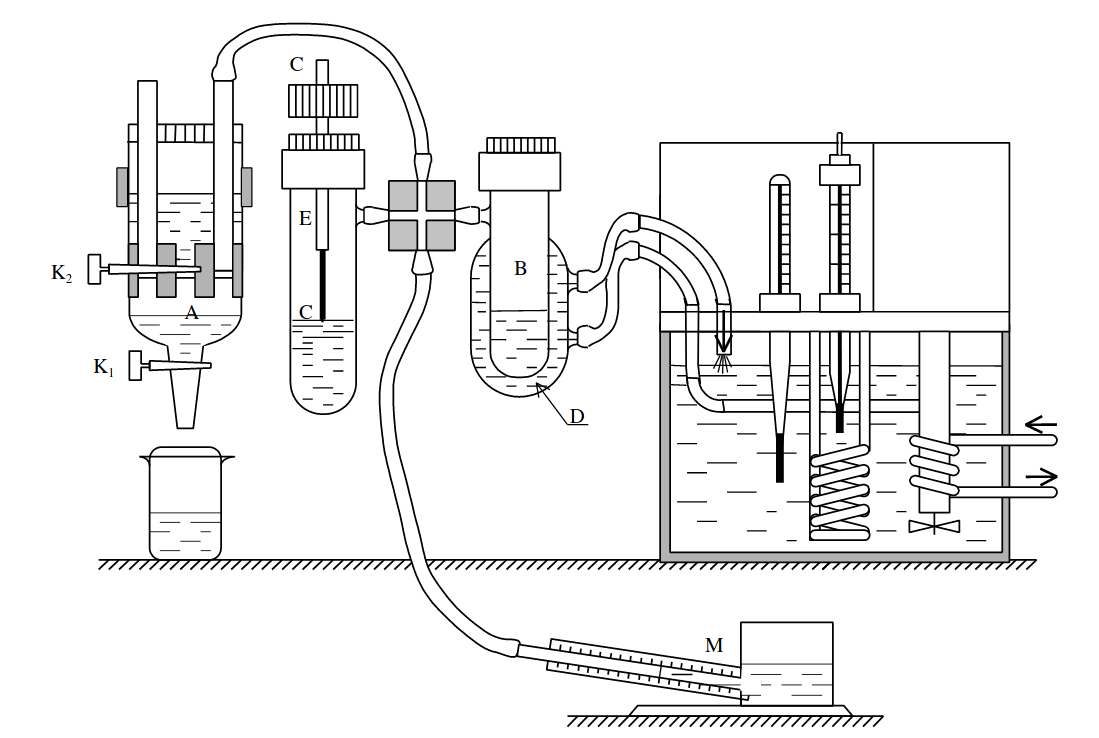
\includegraphics[width=0.9\linewidth]{res/scheme.png}
		\end{center}
		\caption{Схема установки}
		\label{scheme}
	\end{figure}	
	
	
	\section*{Ход работы}
	
	\subsection*{Спирт}
	
		$\quad \;$ Коэффициент пересчета столба спиртового манометра в давление:
		
		$$K_{пер} = 0.2 \cdot 9.81 \cdot 0.8095 = 1.588 \; \text{Па}/\text{мм}$$
	
		Поместим иглу в сосуд со спиртом, закроем пробками сосуды, открыв кран аспиратора добьемся пробулькивания пузырьков воздуха.
		
		\begin{table}[h]
			\caption{Давление пробулькивания в спирте, игла на поверхности}
			\begin{tabular}{|l|lll|}
				$h$, мм & 44 & 44 & 45 \\
			\end{tabular}
		\end{table}
	
	    $$\bar{h} = \frac{\sum\limits_{i=1}^3 h_i}{3}=44.3 \; \text{мм}$$
		$$p = K_{пер} \cdot \bar{h} = 70.4 \; \text{Па}$$
		
		Воспользовавшись табличным значением поверхностного натяжения для спирта:
		
		$$\sigma_{\text{спирта}} = 22 \; \frac{\text{мН}}{\text{мм}}$$
		
		Значения диаметра иглы, измеренные с помощью микроскопа и косвенно:
		
		$$ d_{\text{микр}} = (1.20 \pm 0.05) \; \text{мм} \qquad 
		   d_{\text{косв}} = \frac{4\sigma}{p} =  (1.28 \pm 0.03) \; \text{мм} $$
		При дальнейших расчётах, чтобы учесть особенности данной установки будем использовать d_{\text{косв}}.
		
	\subsection*{Вода}
	
		$\quad$ Измерим давления, при которых начинается пробулькивание.
		
		\begin{table}[H]
			\caption{Давление пробулькивания в водe, игла на поверхности}
			\begin{tabular}{|l|lll|}
				$h_{пов}, \; \text{мм}$ & 74 & 75 & 74    \\
			\end{tabular}
		\end{table}
		
		\begin{table}[H]
			\caption{Давление пробулькивания в воде, игла на глубине}
			\begin{tabular}{|l|lll|}
				$h_{глуб}, \; \text{мм}$ & 196    & 196    & 197    \\
			\end{tabular}
		\end{table}
	
		$$\Delta h = h_1 - h_2 = 23.5 - 11.5 = (12.0 \pm 0.5) \; \text{мм}$$
		
		$$\Delta h = \frac{p_2 - p_1}{\rho g} = \frac{1.588\cdot(196.3 - 74.3)}{9.81\cdot1000} =(17.2 \pm 0.3) \; \text{мм}$$
		Таким образом, дополнительная разность давлений 
		$$\Delta p_{\text{доп}}=\rho g \Delta h = 1000 \cdot 9.81 \cdot 0.0120 = 117.60 \; \text{Па}$$
	
		Формула для определения $\sigma$:
		
		$$ \sigma = \frac{pr}{2},$$
		где $p = \bar{p} - \Delta p_{\text{доп}}$
		$$$$
		Погрешности измерения:
		
		$$\varDelta p = 1.6 \; \text{Па} \qquad \varDelta T = 0.2 \; \text{K} \qquad \varDelta \sigma = \sigma \sqrt{ (\varDelta p / p)^2 + (\varDelta r / r)^2 } = 2 \; \text{Н} / \text{м}$$

		Измерим зависимость давления от температуры.
		
		\begin{table}[h]
			\caption{Зависимость $\overline{p}(T)$}
			\begin{tabular}{cccccccc}
\toprule
$T, ^{\circ} C$ & $h_1, \; \text{мм}$ & $h_2, \; \text{мм}$ & $h_2, \; \text{мм}$ &
$\bar{h}, \; \text{мм}$ & $\bar{p}, \; \text{Па}$ & $p, \; \text{Па}$ & $\sigma_\text{пов}, \; \frac{\text{Н}}{\text{м}}$ \\
\midrule
24.5 & 196 & 196 & 197 & 196.33 & 311.82 & 194.22 & 0.0583 \\
30.3 & 195 & 194 & 194 & 194.33 & 308.65 & 191.05 & 0.0573 \\
35.2 & 193 & 194 & 193 & 193.33 & 307.06 & 189.46 & 0.0568 \\
40.3 & 192 & 191 & 192 & 191.67 & 304.41 & 186.81 & 0.0560 \\
45.2 & 190 & 190 & 190 & 190.00 & 301.77 & 184.17 & 0.0552 \\
50.1 & 189 & 189 & 190 & 189.33 & 300.71 & 183.11 & 0.0549 \\
55.0 & 187 & 188 & 188 & 187.67 & 298.06 & 180.46 & 0.0541 \\
60.0 & 185 & 186 & 186 & 185.67 & 294.88 & 177.28 & 0.0532 \\
65.1 & 185 & 185 & 185 & 185.00 & 293.82 & 176.22 & 0.0529 \\
70.0 & 184 & 183 & 183 & 183.33 & 291.18 & 173.58 & 0.0521 \\
\bottomrule
\end{tabular}
		\end{table}
		
		Построим график.
		
		\begin{figure}[H]
			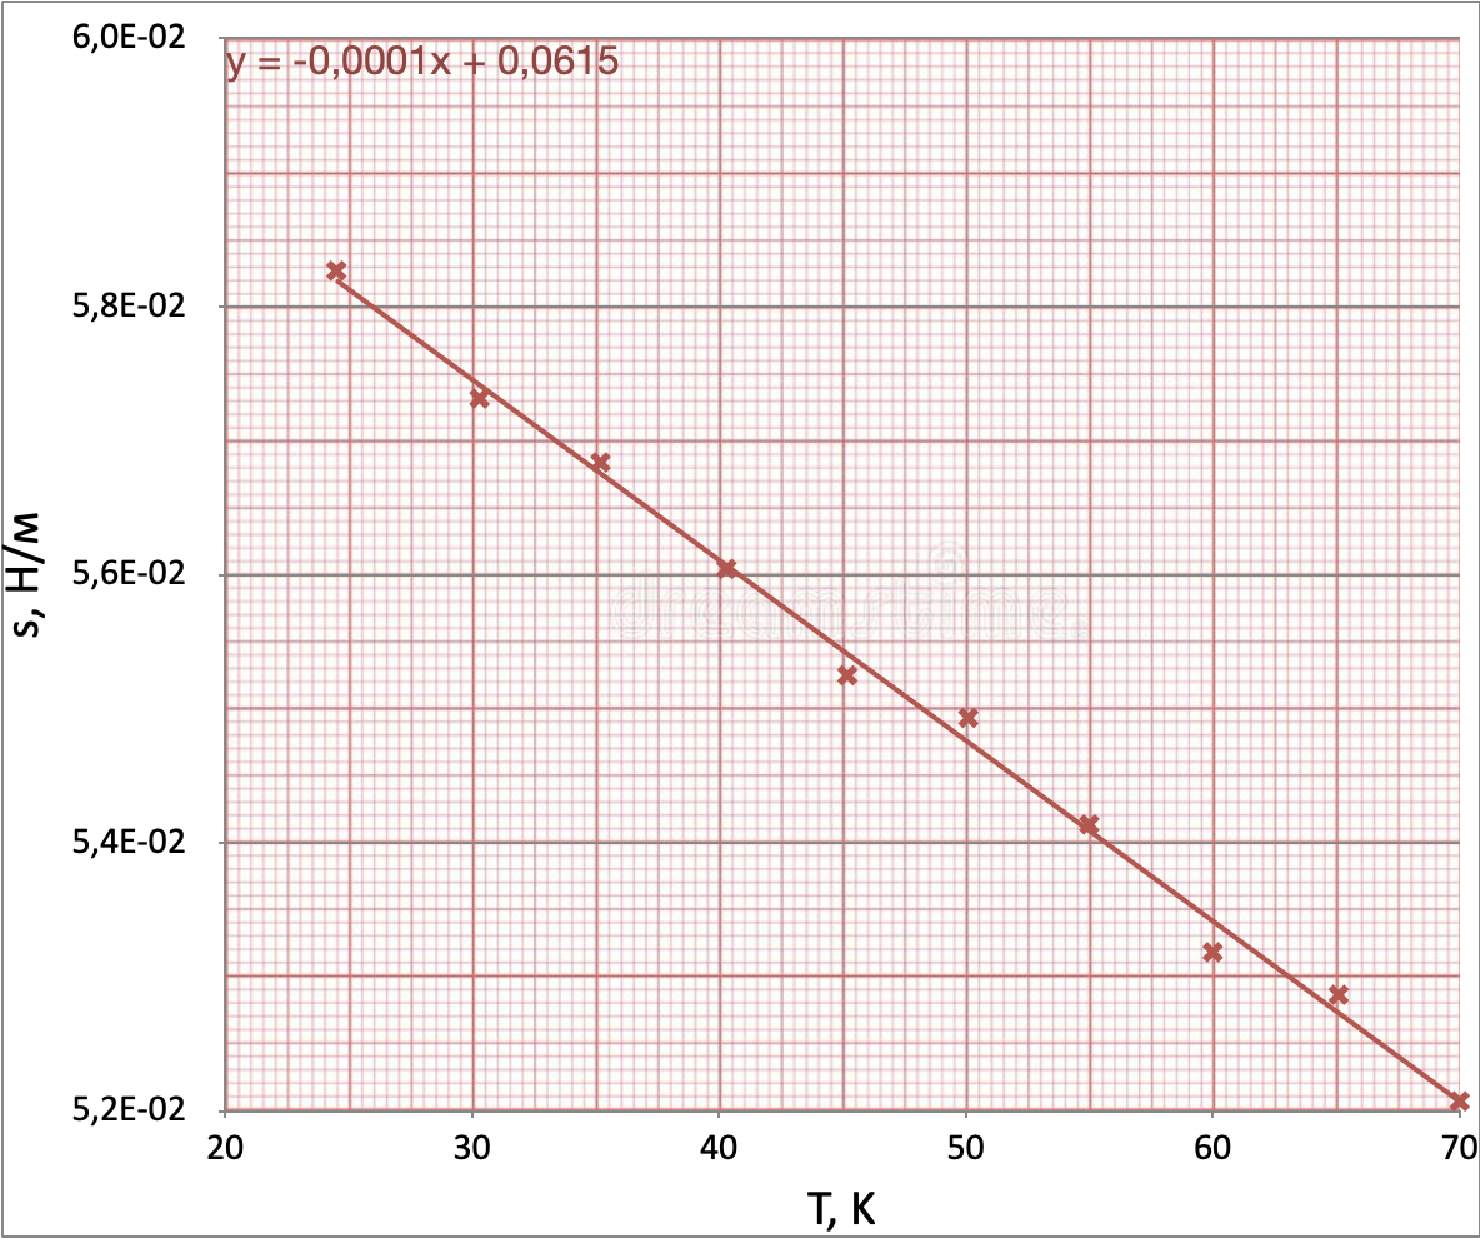
\includegraphics[width = 10.5 cm]{src/s(t).pdf}
			\caption{$ \text{Зависимость} \; \sigma(T)$}
		\end{figure}
		
		
		По методу наименьших квадратов, предполагая зависимость линейной $\sigma_\text{\text{пов}} = a\cdot T + b,$
		
		где
		   $$a=(-1.35 \pm 0.06)\cdot 10^{-4} \; \frac{\text{Н}}{\text{м}\cdot \text{К}} \;\;\;\; \varepsilon_{\gamma}=5\%$$
		   $$b=( 6.15 \pm 0.03)\cdot 10^{-2} \; \frac{\text{Н}}{\text{м}} \;\;\;\; \varepsilon_{\gamma}=0.5\%$$
	

		Также построим графики:
		
		1) теплоты образования единицы поверхности жидкости $q = - T \frac{d\sigma}{dT}$.
		
		2) поверхностной энергии $U$ единицы площади $F$: $\frac{U}{F} = \sigma - T \frac{d\sigma}{dT}$.
	
				
		\begin{figure}[H]
			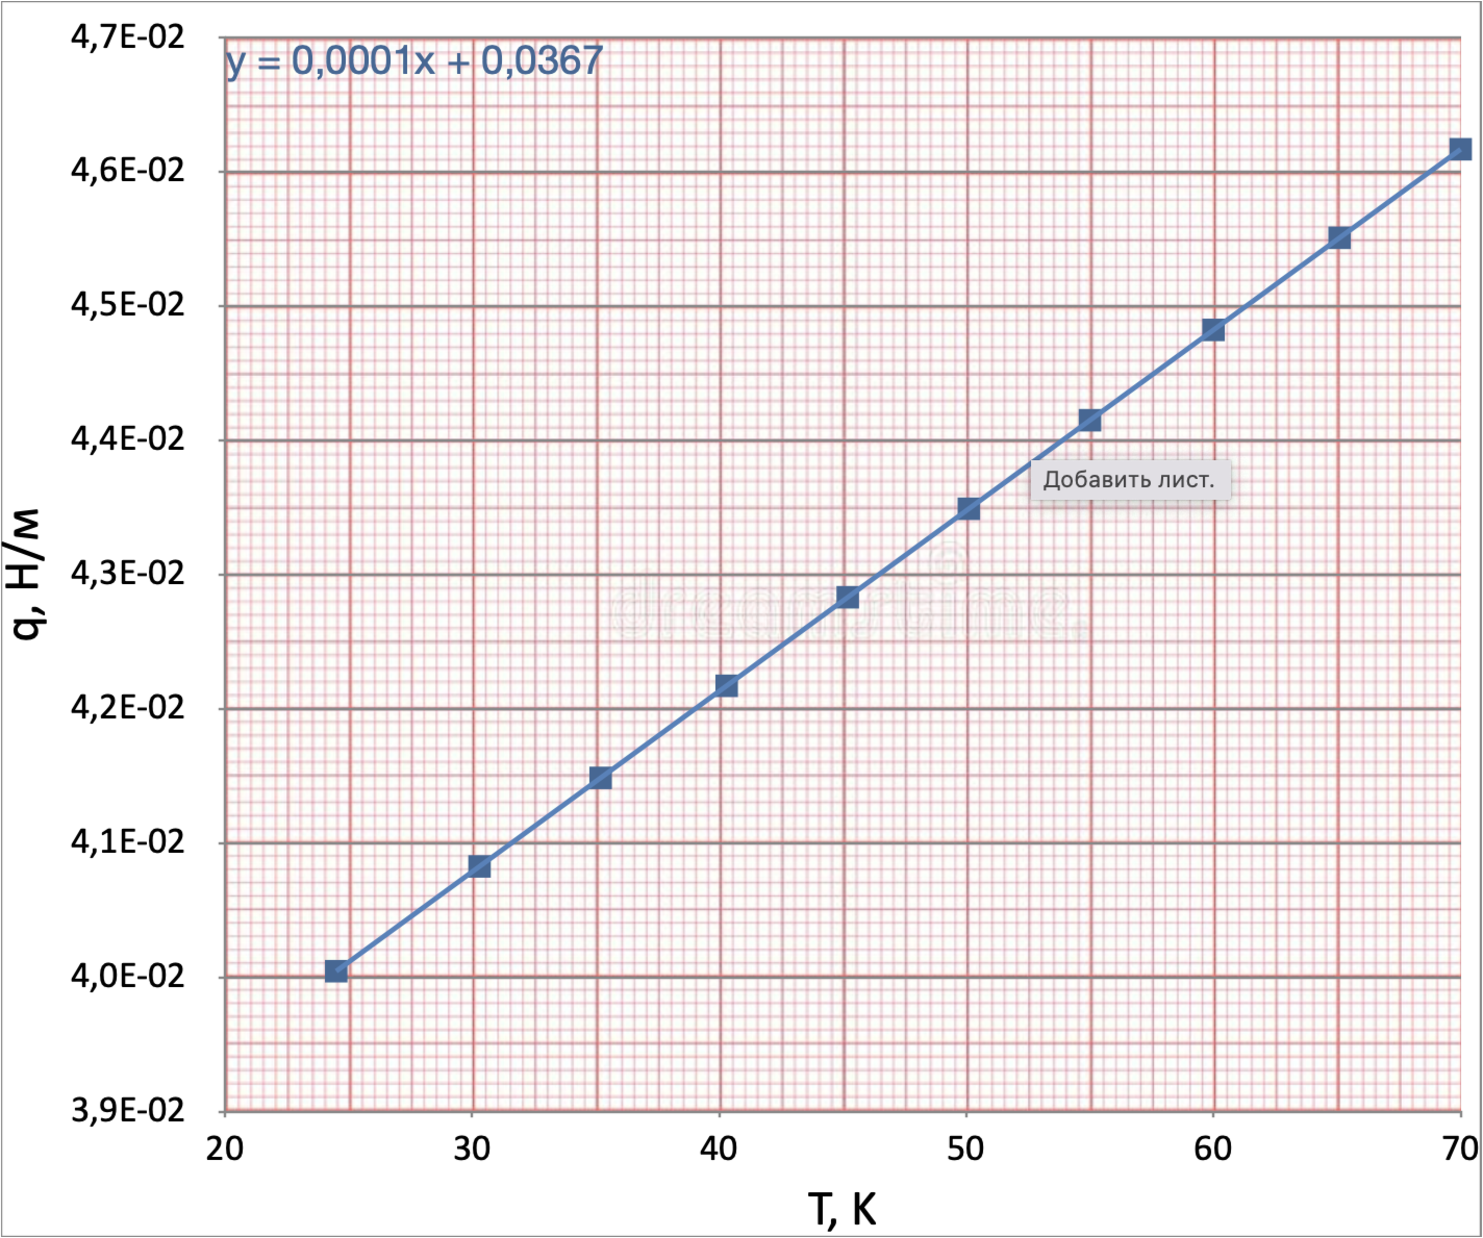
\includegraphics[width = 10.5 cm]{src/q_t.pdf}
			\caption{$ \text{Зависимость} \; q(T)$}
		\end{figure}
		
		\begin{figure}[H]
			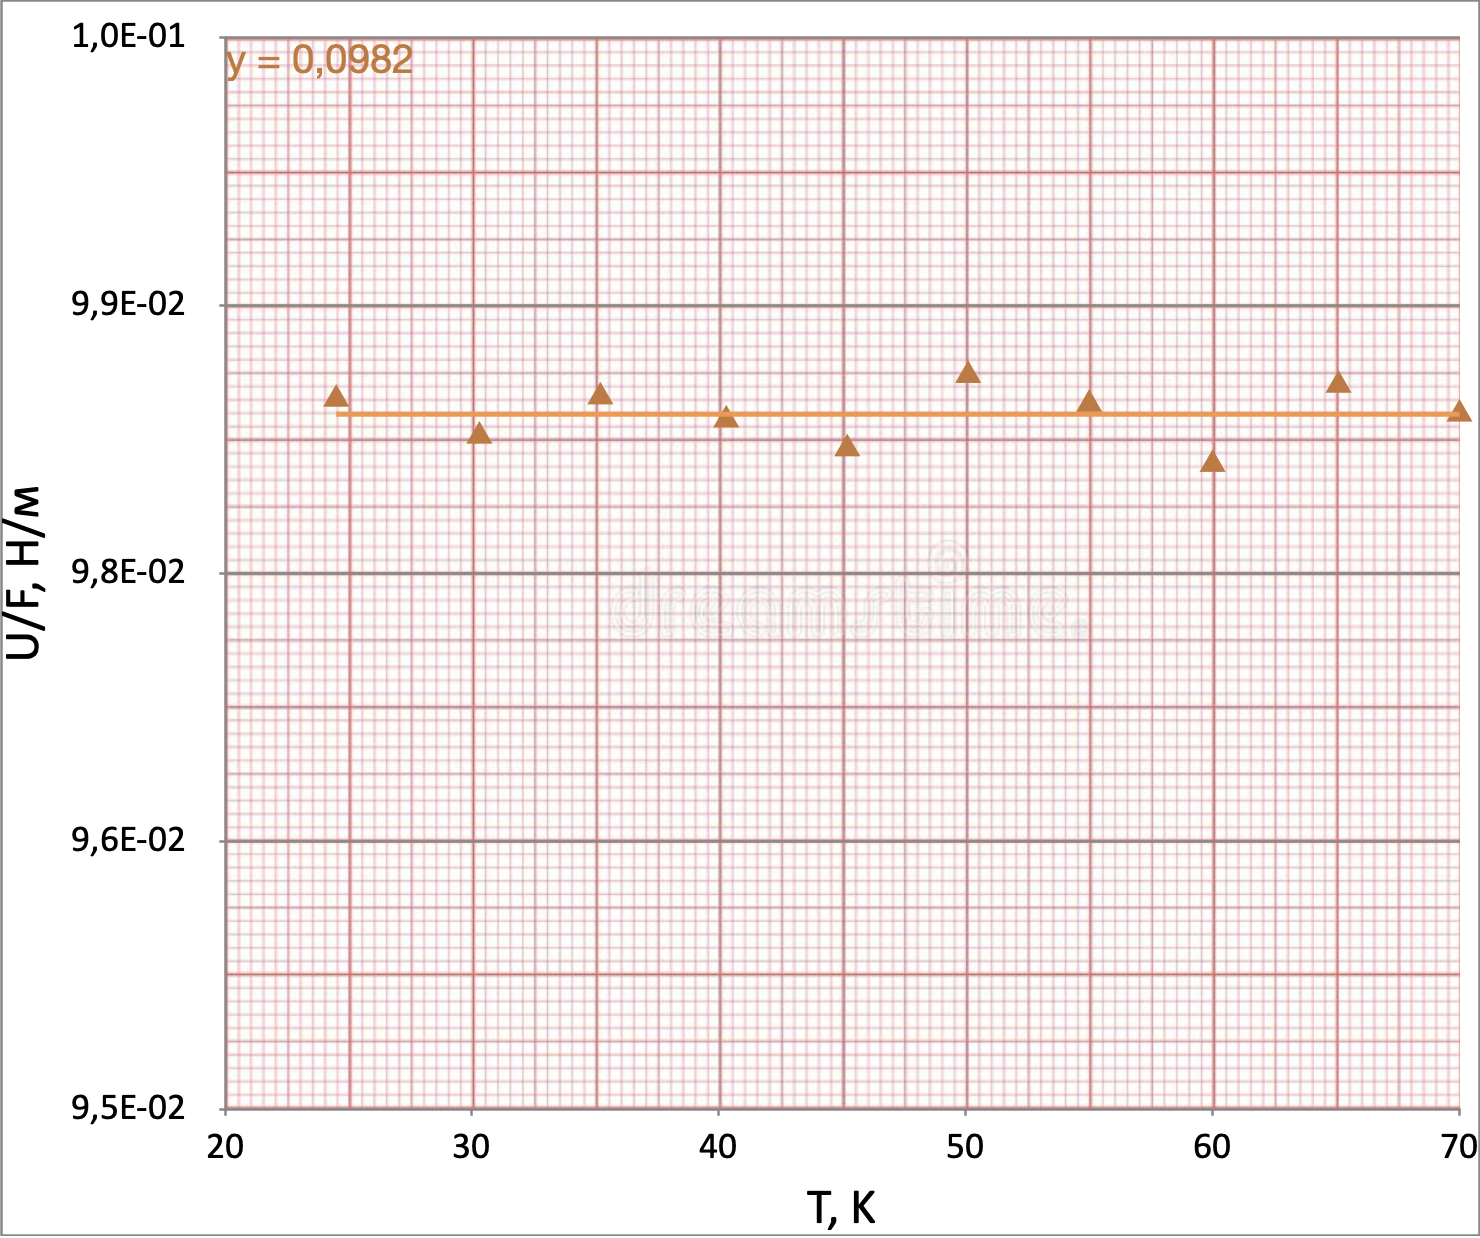
\includegraphics[width = 10.5 cm]{src/u_f_t.pdf}
			\caption{$ \text{Зависимость} \; U/F \;(T)$}
		\end{figure}
		
		\begin{table}[h]
			\caption{Зависимости $q(T), \; U/F(T)$}
			\begin{tabular}{ccc}
\toprule
$T, ^{\circ} C$ & $h_1, \; \text{мм}$ & $q, \; \frac{\text{мН}}{\text{м}}$ & $\frac{U}{F}, \; \frac{\text{мН}}{\text{м}}$ \\
\midrule
24.5 & 40.0 & 98.3 \\
30.3 & 40.8 & 98.1 \\
35.2 & 41.5 & 98.3 \\
40.3 & 42.2 & 98.2 \\
45.2 & 42.8 & 98.1 \\
50.1 & 43.5 & 98.4 \\
55.0 & 44.2 & 98.3 \\
60.0 & 44.8 & 98.0 \\
65.1 & 45.5 & 98.4 \\
70.0 & 46.2 & 98.2 \\
\bottomrule
\end{tabular}
		\end{table}
		
	\section*{Вывод}
	
		$\quad$ В ходе эксперимента была подтверждена линейная зависимость коэффициента поверхностного натяжения от температуры. Однако сами значения поверхностного натяжения от температуры систематически отличаются от табличного 
		$\sigma_{\text{табл}} = 73 \; \text{мН}/\text{м}$
		значения. Отклонение может возникнуть вследствие попадания спирта в пробирку с водой из-за нетщательной просушки иглы в предыдущих экспериментах (спирт имеет $\sigma_{\text{сп}} = 22 \; \text{мН}/\text{м}$, поэтому поверхностное натяжение смеси ниже).
		
		
		Получено значение 
		$$d\sigma/dT)_{\text{эксп}} = (-0.135 \pm 0.06) \; \frac{\text{мН}}{\text{м}\cdot\text{К}} \;\;\;\; \varepsilon_{d\sigma/dT)_{\text{эксп}}}=5\%.$$
		Не сильно отличающееся от табличного
		$(d\sigma/dT)_{\text{табл}} = - 0.15 \; \frac{\text{мН}}{\text{м} \cdot \text{K}}.$
		Также в ходе работы определено значение
		$$\frac{U_{\text{пов}}}{F} = (98.2 \pm 0.3) \; \frac{\text{мН}}{\text{м}}  \;\;\;\; \varepsilon_{\frac{U_{\text{пов}}}{F}}=0.3\%.$$
		Табличное значение $\frac{U_{\text{пов}}}{F} = 120 \; \frac{\text{мН}}{\text{м}}.$
		Показана линейность зависимости $q(T).$
		
\end{document}